\documentclass[10pt,a4paper,footinclude=true,headinclude=true]{scrbook}

\newcommand{\myName}{Alessandro Candolini}
\newcommand{\myTitle}{Short treatise on the mathematical theory of monoidal categories}
\newcommand{\myLocation}{London}
\newcommand{\myTime}{\today}

% *****************************************************************************
%  Main packages
% *****************************************************************************

\usepackage[T1]{fontenc}
\usepackage[applemac]{inputenc}
\usepackage[english]{babel}
\usepackage[babel]{csquotes}
\usepackage{graphicx}
\usepackage[dvipsnames]{xcolor}


% typography
\usepackage[hyphenation]{impnattypo}
\usepackage[biblatex=true]{embrac}
\usepackage[final]{microtype}

\usepackage{listings}

\usepackage{makeidx}

\usepackage{tabularx}
\usepackage{booktabs}
\usepackage{subfig}
\usepackage{sidecap}
\usepackage{url}
\usepackage[font=small, noorphanfirst, indentfirst=false]{quoting}



% *****************************************************************************
% BIBLaTeX
% *****************************************************************************
\usepackage[%
style=philosophy-modern,
%style=philosophy-classic,
scauthorsbib,
hyperref,backref,
backend=biber,
square,
natbib,ibidtracker=false]{biblatex}

\bibliography{myBibliography9}

% ClassicThesis
\usepackage[pdfspacing,
  eulerchapternumbers,
  listings,
  eulermath,
  %style=arsclassica,
  parts,
  floatperchapter]{classicthesis}


% Footnote
\usepackage[perpage, symbol*, stable, multiple]{footmisc}
\setlength{\footnotemargin}{.6em}%

\usepackage{fnpct}
\setfnpct{add-punct-marks=:}
\setfnpct{add-punct-marks=;}

\usepackage{footnotebackref}
\makeatletter
\ifx\c@Hfootnote\undefined
\newcounter{Hfootnote}%
\fi

  \let\H@@footnotetext\@footnotetext
  \let\H@@footnotemark\@footnotemark
  \def\@xfootnotenext[#1]{%
    \begingroup
      \csname c@\@mpfn\endcsname #1\relax
      \unrestored@protected@xdef\@thefnmark{\thempfn}%
    \endgroup
    \ifx\@footnotetext\@mpfootnotetext
      \expandafter\H@@mpfootnotetext
    \else
      \expandafter\H@@footnotetext
    \fi
  }%
  \def\@xfootnotemark[#1]{%
    \begingroup
      \c@footnote #1\relax
      \unrestored@protected@xdef\@thefnmark{\thefootnote}%
    \endgroup
    \H@@footnotemark
  }%
  \let\H@@mpfootnotetext\@mpfootnotetext
  \long\def\@mpfootnotetext#1{%
    \H@@mpfootnotetext{%
      \ifHy@nesting
        \expandafter\hyper@@anchor\expandafter{%
          \Hy@footnote@currentHref
         }{#1}%
      \else
        \Hy@raisedlink{%
          \expandafter\hyper@@anchor\expandafter{%
            \Hy@footnote@currentHref
          }{\relax}%
        }#1%
      \fi
    }%
  }%
  \long\def\@footnotetext#1{%
    \H@@footnotetext{%
      \ifHy@nesting
        \expandafter\hyper@@anchor\expandafter{%
          \Hy@footnote@currentHref
        }{#1}%
      \else
        \Hy@raisedlink{%
          \expandafter\hyper@@anchor\expandafter{%
            \Hy@footnote@currentHref
          }{\relax}%
        }%
        \let\@currentHref\Hy@footnote@currentHref
        \let\@currentlabelname\@empty
        #1%
      \fi
    }%
  }%
  \def\@footnotemark{%
    \leavevmode
    \ifhmode\edef\@x@sf{\the\spacefactor}\nobreak\fi
    \stepcounter{Hfootnote}%
    \global\let\Hy@saved@currentHref\@currentHref
    \hyper@makecurrent{Hfootnote}%
    \global\let\Hy@footnote@currentHref\@currentHref
    \global\let\@currentHref\Hy@saved@currentHref
    \hyper@linkstart{link}{\Hy@footnote@currentHref}%
    \@makefnmark
    \hyper@linkend
    \ifhmode\spacefactor\@x@sf\fi
    \relax
  }%


\long\def\@footnotetext#1{%
      \H@@footnotetext{%
        \ifHy@nesting
         \hyper@@anchor{\@currentHref}{#1}%
       \else
         \Hy@raisedlink{\hyper@@anchor{\@currentHref}{\relax}}#1%
       \fi
     }}


  \def\@footnotemark{%
     \leavevmode
     \ifhmode\edef\@x@sf{\the\spacefactor}\nobreak\fi
     \H@refstepcounter{Hfootnote}%
     \hyper@makecurrent{Hfootnote}%
     \hyper@linkstart{link}{\@currentHref}%
     \@makefnmark
     \hyper@linkend
     \ifhmode\spacefactor\@x@sf\fi
     \relax
   }%

 \ifFN@multiplefootnote%
     \renewcommand*\@footnotemark{%
      \leavevmode
      \ifhmode
        \edef\@x@sf{\the\spacefactor}%
        \FN@mf@check
        \nobreak
      \fi
      \H@refstepcounter{Hfootnote}%
      \hyper@makecurrent{Hfootnote}%
      \hyper@linkstart{link}{\@currentHref}%
      \@makefnmark
      \hyper@linkend
      \FN@mf@prepare
      \ifhmode\spacefactor\@x@sf\fi
      \relax%
    }%
 \fi

\makeatother




\newenvironment{citazione}%
  {\begin{quotation}\small\ignorespaces}%
  {\end{quotation}}
\newenvironment{approfondimento}%
  {\begin{quotation}\small\ignorespaces}%
  {\end{quotation}}

\graphicspath{{./},{./Asymptote/}, {./Images/}}

% i.e.
\newcommand{\ie}{i.\,e.}
\newcommand{\Ie}{I.\,e.}
\newcommand{\eg}{e.\,g.}
\newcommand{\Eg}{E.\,g.}


% ********************************************************************
% hyperref
% ********************************************************************
\hypersetup{%
    colorlinks=true, linktocpage=true, pdfstartpage=1, pdfstartview=FitV,%
    breaklinks=true, pdfpagemode=UseNone, pageanchor=true, pdfpagemode=UseOutlines,%
    plainpages=false, bookmarksnumbered, bookmarksopen=true, bookmarksopenlevel=1,%
    hypertexnames=true, pdfhighlight=/O,%
    urlcolor=webbrown, linkcolor=RoyalBlue, citecolor=RoyalBlue,citecolor=webgreen,
    pdftitle={\myTitle},%
    pdfauthor={\textcopyright\ \myName},%
    pdfsubject={},%
    pdfkeywords={},%
    pdfcreator={pdfLaTeX},%
    pdfproducer={LaTeX con hyperref e ClassicThesis}%
}

\newcommand{\mail}[1]{\href{mailto:#1}{\texttt{#1}}}


% *****************************************************************************
% Math
% *****************************************************************************

% AMSmath packages
\usepackage{amssymb}

% comandi per gli insiemi numerici (serve il pacchetto amssymb)
\newcommand{\numberset}{\mathbb}
\newcommand{\N}{\numberset{N}}
\newcommand{\Z}{\numberset{Z}}
\newcommand{\Q}{\numberset{Q}}
\newcommand{\R}{\numberset{R}}
\newcommand{\C}{\numberset{C}}

\usepackage{braket}
\usepackage{cool}

% Theorems
\usepackage{amsthm}

\makeatletter
\newtheoremstyle{classicdef}%
{11pt}%                                   % Before
{11pt}%                                   % After
{}%                                       % Font
{}%                                       % Rientro (se vuoto, nessun rientro;
%                                         % \parindent = rientro dei capoversi)
{\scshape}%                               % Font
{:}%
{.5em}%
{}%
\makeatother

\theoremstyle{classicdef}
\newtheorem{theorem}{Theorem}[chapter]
\newtheorem{lemma}{Lemma}[chapter]
\newtheorem{definition}{Definition}[chapter]
\newtheorem*{homework}{Homework}
\theoremstyle{remark}
\newtheorem*{remark}{Remark}
\renewcommand{\qedsymbol}{\rule{.5em}{.5em}}


\usepackage{caption}                      % Fancy captions and more.
\captionsetup{format=hang,font=small}
\captionsetup[table]{skip=\medskipamount}

\usepackage{mathtools}
\usepackage{flexisym}
\usepackage{breqn}
\DeclareFlexSymbol{\Gamma}  {Var}{latin}{00}
\DeclareFlexSymbol{\Delta}  {Var}{latin}{01}
\DeclareFlexSymbol{\Theta}  {Var}{latin}{02}
\DeclareFlexSymbol{\Lambda} {Var}{latin}{03}
\DeclareFlexSymbol{\Xi}     {Var}{latin}{04}
\DeclareFlexSymbol{\Pi}     {Var}{latin}{05}
\DeclareFlexSymbol{\Sigma}  {Var}{latin}{06}
\DeclareFlexSymbol{\Upsilon}{Var}{latin}{07}
\DeclareFlexSymbol{\Phi}    {Var}{latin}{08}
\DeclareFlexSymbol{\Psi}    {Var}{latin}{09}
\DeclareFlexSymbol{\Omega}  {Var}{latin}{0A}
\DeclareFlexSymbol{0}{Var}{latin}{30}
\DeclareFlexSymbol{1}{Var}{latin}{31}
\DeclareFlexSymbol{2}{Var}{latin}{32}
\DeclareFlexSymbol{3}{Var}{latin}{33}
\DeclareFlexSymbol{4}{Var}{latin}{34}
\DeclareFlexSymbol{5}{Var}{latin}{35}
\DeclareFlexSymbol{6}{Var}{latin}{36}
\DeclareFlexSymbol{7}{Var}{latin}{37}
\DeclareFlexSymbol{8}{Var}{latin}{38}
\DeclareFlexSymbol{9}{Var}{latin}{39}


\setkeys{breqn}{labelprefix={eq:}}


% Cleveref
\usepackage{cleveref}
\crefname{chapter}{\S}{\S}
\Crefname{chapter}{\S}{\S}
% *****************************************************************************
% Main
% *****************************************************************************
\begin{document}
\pagenumbering{roman}
\pagestyle{plain}
\begin{titlepage}
	\begin{addmargin}[-1cm]{-3cm}
    \begin{center}
{
        \large

        \hfill

        \vfill

        \begingroup
            \color{Maroon}\spacedallcaps{\myTitle} \ \bigskip
        \endgroup

        \spacedlowsmallcaps{\myName}

        \vfill

\vfill
}
	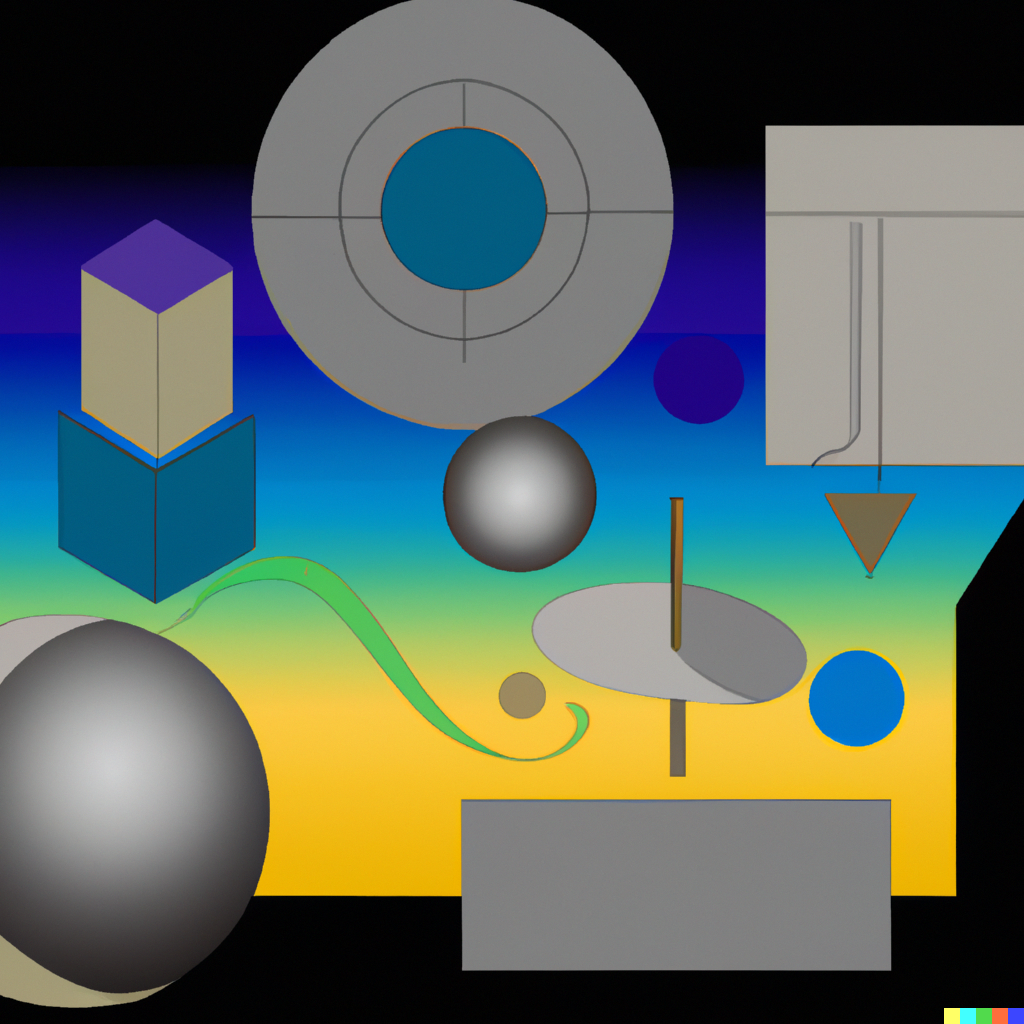
\includegraphics[width=.9\textwidth]{cover}
	\vspace{\stretch{5}}


        \textsw{\myTime}
    \end{center}
  \end{addmargin}
\end{titlepage}

\thispagestyle{empty}

\hfill

\vfill

\noindent\myName: \textit{\myTitle}
\textcopyright\ \MakeTextLowercase{\myTime}.

\medskip
\medskip
\noindent{\spacedlowsmallcaps{E-mail}}: \
\mail{alessandro.candolini@gmail.com}

\vspace{1cm}
\bigskip

%*******************************************************
% Dedication
%*******************************************************
\cleardoublepage
\thispagestyle{empty}
\pdfbookmark[1]{Dedica}{Dedica}

\vspace*{3cm}

\selectlanguage{english}
\begin{quotation}
%   \openquote 
  There is nothing more practical than a good theory.%~\closequote
\begin{flushright}
    --- Kurt Lewin, 1945 
\end{flushright}
%\end{center}
\end{quotation}

\pagestyle{scrheadings}
\cleardoublepage
\phantomsection
\pdfbookmark{\contentsname}{tableofcontents}
\setcounter{tocdepth}{2}
\tableofcontents
\markboth{\spacedlowsmallcaps{\contentsname}}{\spacedlowsmallcaps{\contentsname}} 

\cleardoublepage


\chapter*{Reflections on category theory}
\markboth{\spacedlowsmallcaps{Preface}}{\spacedlowsmallcaps{Preface}}
\addcontentsline{toc}{chapter}{\tocEntry{Preface}}


These notes provide an exploration of concepts and ideas in category theory, with special emphasis on various flavours of monoidal categories, with applications to algebra, non-relativistic quantum mechanics, and applied functional programming. 

Category theory recently has gained prominence in several areas of pure and applied mathematics, physics, and computer science. 
Due to its extreme generality and versatility, category theory offers a unifying framework through which a wide variety of topics can be recast and understood.  
A question arises though, on whether that's just an exercise of purely theoretical interested, or there are compelling advantages over more traditional approaches. 
%Personally, I don't think there's a unique and straightforward answer to this question, but 
In challenging and stimulating a discussion around this question, 
these notes contribute by offering a gallery of domains and examples where looking through the eyeglass of category theory unlocks new ways of reasonings, provides a bird-eye view that allows to connect seemigly unrelated areas, and suggestively inspire new insightful ways to look at existing domains. 
In fact, category theory provides a conceptual and theoretical framework and language to express, develop, and reason about abstractions and domains in a general manner that often allows to remove the accidental complexity, noisy ``implementation details'', and unnecessary burden of more traditional formalisms, letting the core aspects and essential properties emerge. 

Consider, for instance, the operatorial formulation of non-relativistic quantum mechanics, due to von Neumann, based on the spectral theory of linear self-adjoint operators on Hilbert spaces. (Alternative formulations, such as the path integral approach introduced by R.~Feynman, offer valuable physical insights but play a more prominent role in perturbative relativistic quantum field theories.) Despite the undeniable usefulness and effectiveness of the operatorial formalism in describing and calculating properties of various quantum systems, the extraction and recognition of general results are often obfuscated behind a layer of technical details. We will see that results such as the no-cloning theorem, foundational in quantum computation and usually derived using the Cauchy-Schwarz inequality for Hilbert spaces, emerge naturally from the structural constraints of dagger compact categories.

%Consider, for instance, the operatorial formulation of non-relativistic quantum mechanics --- which goes back to von Neumann --- in terms of spectral theory of linear self-adjoint operators in Hilbert spaces. This formalism has proven to be particularly suitable and powerful to describe and extract properties of quantum systems. (Alternative formulations include the usage of path integrals, due to R.~Feynman; while such approach is interesting and insighful from a physical viewpoint, it shines in the perpurbative treatment of relativistic quantum field theories.). Despite the undeniable usefulness and effectiveness of the operatorial formalism in describing quantum systems, general properties end up often being obfuscated by the details of this construction. We will see that results like the no-cloning theorem, important in quantum computation and whose traditional proof is usually deeply rooted in unitary operators and Hilber spaces of quantum states, emerge naturally from the incompatibility with the structural constraints of dagger compact categories. 

This is not to say that category theory is always suitable for all kind of tasks. 
We need to learn how to resist the pressing temptation of abusing category theory when alternative formulations might provide a better or more effectful alternative.  
Sometimes, in applying quantum mechanics or programming ideas to specific systems or specific code, our goal is exactly to deal with the particularities of such sustems. 
Category theory might not be always the right tool to get our hands dirty when it comes to study the nitty gritty details, mostly because those are often intentionally left ``invisible'' in the categorical construction. From this point of view, category theory should not be understood as a replacement of more traditional approaches. 
Instead, 
wearing the hat of a category theorist provides a complementary viewpoint where certain properties are more naturally expressed, explored, or discovered. 

\smallskip

\noindent\textsw{\myLocation, \myTime}


\begin{flushright}
        \myName
\end{flushright}


\cleardoublepage
\pagenumbering{arabic}
\chapter{Categories}
\label{chap:chap1}


\section{Definition of category}

This is chapter 1.
\begin{dmath}
E = mc^2
\end{dmath}

\chapter{Chapter 2}
\label{chap:chap2}

This is chapter 2.
\begin{dmath}
E = mc^2
\end{dmath}

\chapter{Chapter 3}
\label{chap:chap3}

This is chapter 3.
\begin{dmath}
E = mc^2
\end{dmath}

\appendix
\chapter{Appendix A}


\cleardoublepage
\printbibliography

\cleardoublepage
\manualmark
\markboth{\spacedlowsmallcaps{\indexname}}{\spacedlowsmallcaps{\indexname}}
\phantomsection
\begingroup 
    \let\clearpage\relax
    \let\cleardoublepage\relax
    \let\cleardoublepage\relax
\addcontentsline{toc}{chapter}{\tocEntry{\indexname}}
\printindex
\endgroup 

\end{document}
